%%%%%%%%%%%%%%%%%%%%%%%%%%%%%%%
%%Derived from:
%  ~/LaTeX/beamer/examples/conference-talks/conference-ornate-20min.en.tex
%
%%%%%%%%%%%%%%%%%%%%%%%%%%%%%%%%%%%%%%



\documentclass{beamer}

%%%%%%%%%%%%%%%%%%%
% BEAMER CHOICES
%%%%%%%%%%%%%%%%%%%

\mode<presentation>
{
  \usetheme{Warsaw}
  \setbeamercovered{transparent}
  % or whatever (possibly just delete it)
}

%%%%%%%%%%%
% PACKAGES
%%%%%%%%%%%

\usepackage[english]{babel}
\usepackage[latin1]{inputenc}
\usepackage{times}
\usepackage[T1]{fontenc}

\usepackage{comment}
\usepackage{amsmath}
\usepackage{amsthm}                           % Required for theorem environments
\usepackage{bm}                               % Required for bold math symbols (used in the footer of the slides)
\usepackage{graphicx}                         % Required for including images in figures
\usepackage{booktabs}                         % Required for horizontal rules in tables
\usepackage{multicol}                         % Required for creating multiple columns in slides
\setlength{\columnsep}{0.1mm}
\usepackage{lastpage}                         % For printing the total number of pages at the bottom of each slide
\usepackage{microtype}                        % Better typography
\usepackage{tocstyle}                         % Required for customizing the table of contents
\usepackage{caption}
\captionsetup{labelformat=empty,labelsep=none}
\usepackage{mathtools}
\usepackage{subcaption}
\usepackage{nicefrac}
\usepackage{csquotes}

\usepackage{enumitem}	                        %spread enumeration over multiple slides
\usepackage{pdfpages}
\usepackage{tikz}  
\usepackage[absolute, overlay]{textpos}      %position textblocks (absolute) on the page
\setlength{\TPHorizModule}{\textwidth}
\setlength{\TPVertModule}{\textwidth}



%%%%%%%%%%%%%%%%%%%%%%%%%%%%%%%
% TITLE PAGE AND BEAMER OPTIONS
%%%%%%%%%%%%%%%%%%%%%%%%%%%%%%%%

\title[Short Paper Title] % (optional, use only with long paper titles)
{Title As It Is In the Proceedings}

\subtitle
{Include Only If Paper Has a Subtitle}

\author[Author, Another] % (optional, use only with lots of authors)
{F.~Author\inst{1} \and S.~Another\inst{2}}
% - Give the names in the same order as the appear in the paper.
% - Use the \inst{?} command only if the authors have different
%   affiliation.

\institute[Universities of Somewhere and Elsewhere] 
{
  \inst{1}%
  Department of Computer Science\\
  University of Somewhere
  \and
  \inst{2}%
  Department of Theoretical Philosophy\\
  University of Elsewhere
  }

\date[CFP 2003] % (optional, should be abbreviation of conference name)
{Conference on Fabulous Presentations, 2003}
% - Either use conference name or its abbreviation.


\subject{Theoretical Computer Science}
% This is only inserted into the PDF information catalog. Can be left
% out. 

\pgfdeclareimage[height=0.5cm]{university-logo}{graphics/psulogo_horiz_msword-eps-converted-to.pdf}
\logo{\pgfuseimage{university-logo}}



\AtBeginSubsection[]                                     % the table of contents pops up at the beginning of each subsection
{
  \begin{frame}<beamer>{Outline}
    \tableofcontents[currentsection,currentsubsection]
  \end{frame}
}


%\beamerdefaultoverlayspecification{<+->}              % uncover everything in a step-wise fashion



%%%%%%%%%%%%%%%%%%%%%%%%%
% SPECIALTY NEW COMMANDS
%%%%%%%%%%%%%%%%%%%%%%%%%%
 
% Arrow over vector
\newcommand{\amsvect}{%
  \mathpalette {\overarrow@\vectfill@}}
\def\vectfill@{\arrowfill@\relbar\relbar{\raisebox{-3.81pt}[\p@][\p@]{$\mathord\mathchar"017E$}}}


% Nice-looking fractions
\newcommand\ddfrac[2]{\frac{\displaystyle #1}{\displaystyle #2}}





%#############
%  SLIDES
%#############


\begin{document}

%---------------------------------
\begin{frame}
  \titlepage
\end{frame}

%-----------------------------------
\begin{frame}{Outline}
  \tableofcontents
  % You might wish to add the option [pausesections]
\end{frame}

%----------------------------------
\section{Motivation}
\subsection{The Basic Problem That We Studied}


%---------------------------------------------------
\begin{frame}{Make Titles Informative. Use Uppercase Letters.}{Subtitles are optional.}

\begin{tikzpicture}[overlay]
  \node[anchor=south west] at (5.5,-5.5) {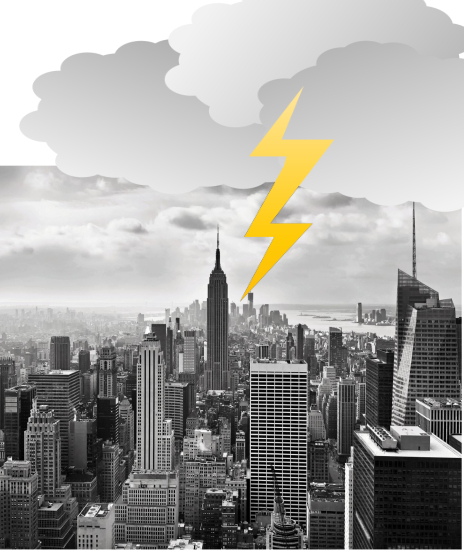
\includegraphics[scale=.45]{graphics/lightning1.jpeg}};  
 \end{tikzpicture}
 
\begin{textblock}{1}(.05,.21)
  \normalsize {Can cityscapes \textbf{influence} weather?}
\end{textblock}

\end{frame}

%--------------------------------------------------------------
\begin{frame}
\begin{tikzpicture}[overlay]
  \node[anchor=south west] at (5.5,-5.5) {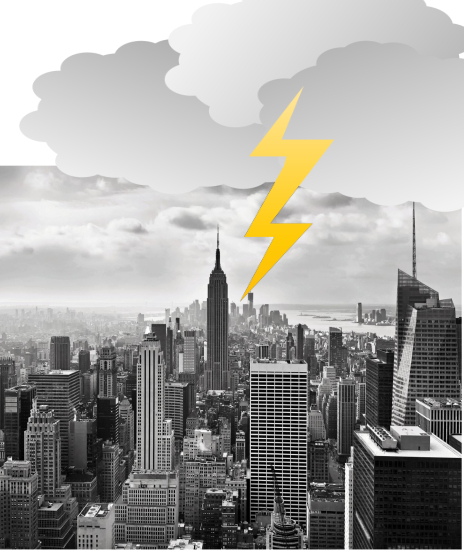
\includegraphics[scale=.45]{graphics/lightning1.jpeg}};  
 \end{tikzpicture}
 
\begin{textblock}{1}(.05,.21)
  \normalsize {Can cityscapes \textbf{influence} weather?}
\end{textblock}
 

\begin{textblock}{1}(.125,.26)
  \normalsize {Can cityscapes \textbf{generate} weather?}
\end{textblock}
\end{frame}

%---------------------------------------------------------------
\begin{frame}
\begin{tikzpicture}[overlay]
  \node[anchor=south west] at (5.5,-5.5) {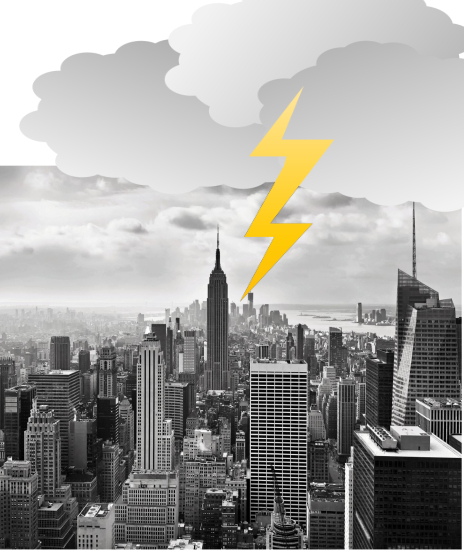
\includegraphics[scale=.45]{graphics/lightning1.jpeg}};  
 \end{tikzpicture}
 
\begin{textblock}{1}(.05,.21)
  \normalsize {Can cityscapes \textbf{influence} weather?}
\end{textblock}
 

\begin{textblock}{1}(.125,.26)
  \normalsize {Can cityscapes \textbf{generate} weather?}
\end{textblock}
 
  
\begin{textblock}{1}(.225,.31)
  \normalsize {Can cityscapes \textbf{cause} thunderstorms?}
\end{textblock}
\end{frame}


%-------------------------------------------------------------------
\begin{frame}{The logic of science: From Reality to models and back again}

\begin{tikzpicture}[overlay]
  \node[anchor=south west] at (6.25,-3.5) {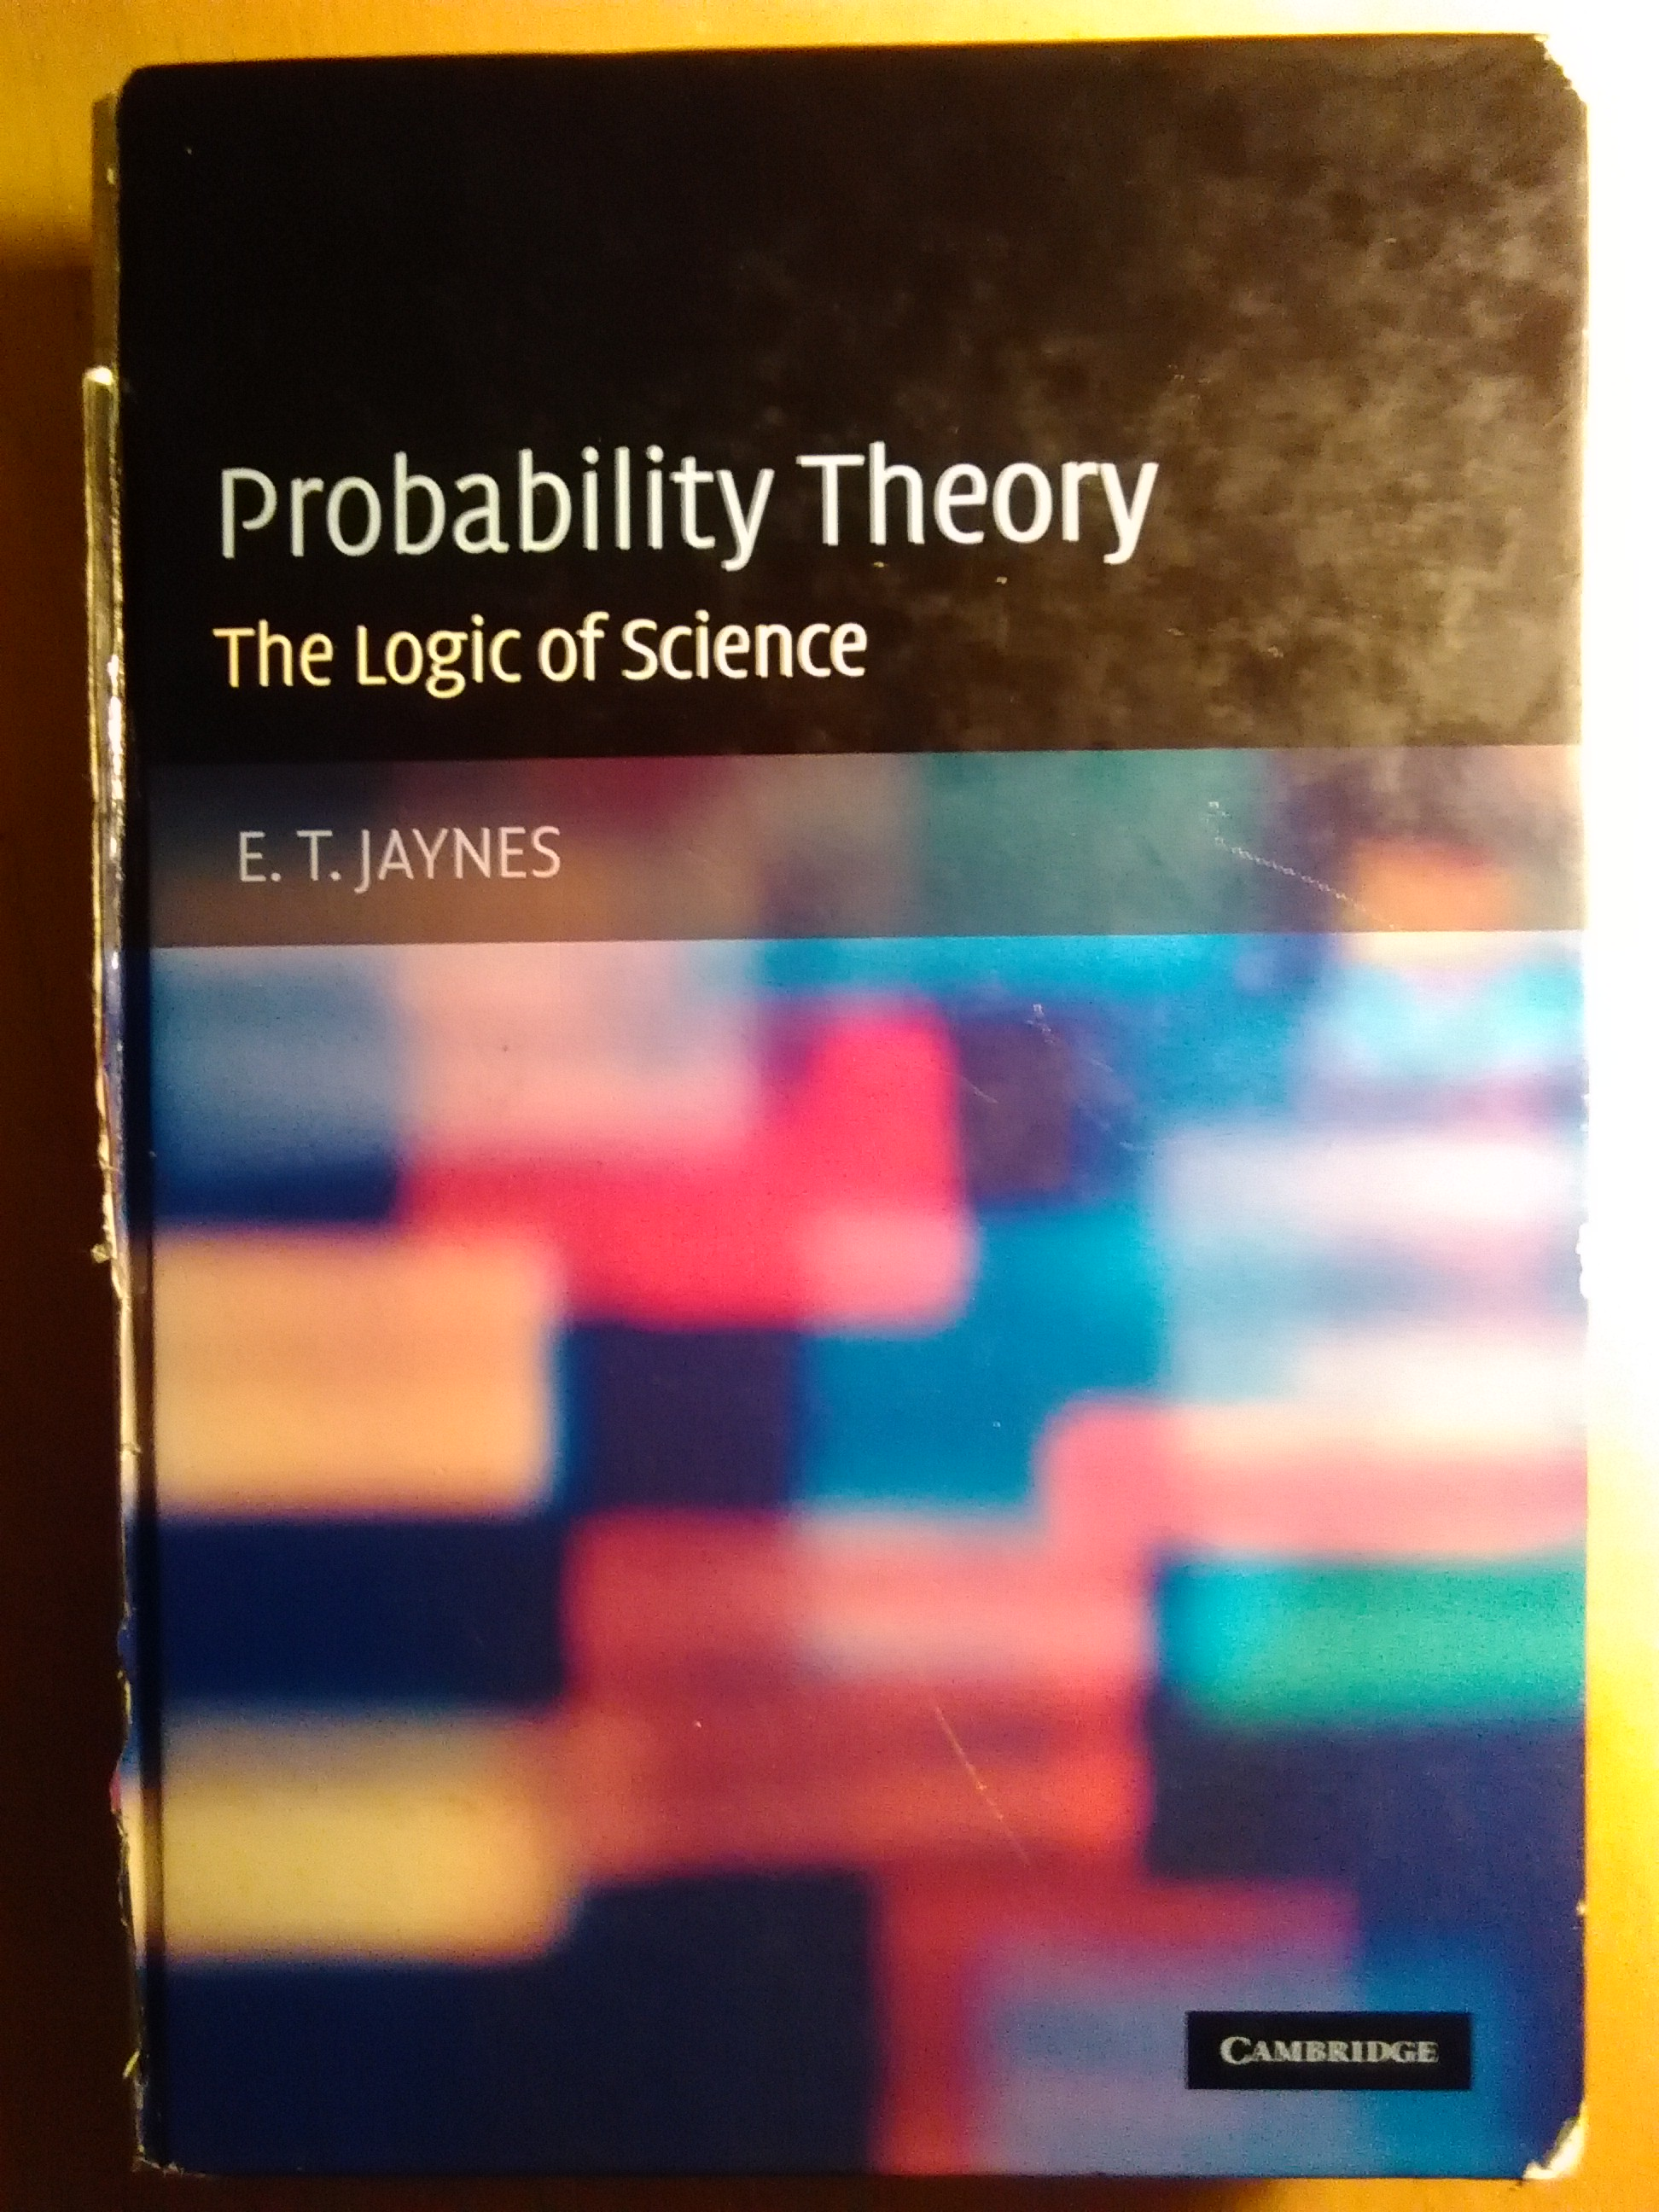
\includegraphics[scale=.070]{graphics/Jaynes.jpg}};  
 \end{tikzpicture}
 
\begin{textblock}{1}(.045,.40)
  \small {"In virtually all real problems of scientific \\
  inference...the problem facing the scientist \\
  is of the inverse type: Given the data D, \\
  what is the probability that some \\
  hypothesis H is true?"}
\end{textblock}

\begin{textblock}{1}(.2,.60)
  \tiny {--- E.T. Jaynes (2003, p.85)}
\end{textblock}

\end{frame}


%----------------------------------------------------------------
\begin{frame}

\begin{tikzpicture}[overlay]
  \node[anchor=south west] at (1.25,-5.5) {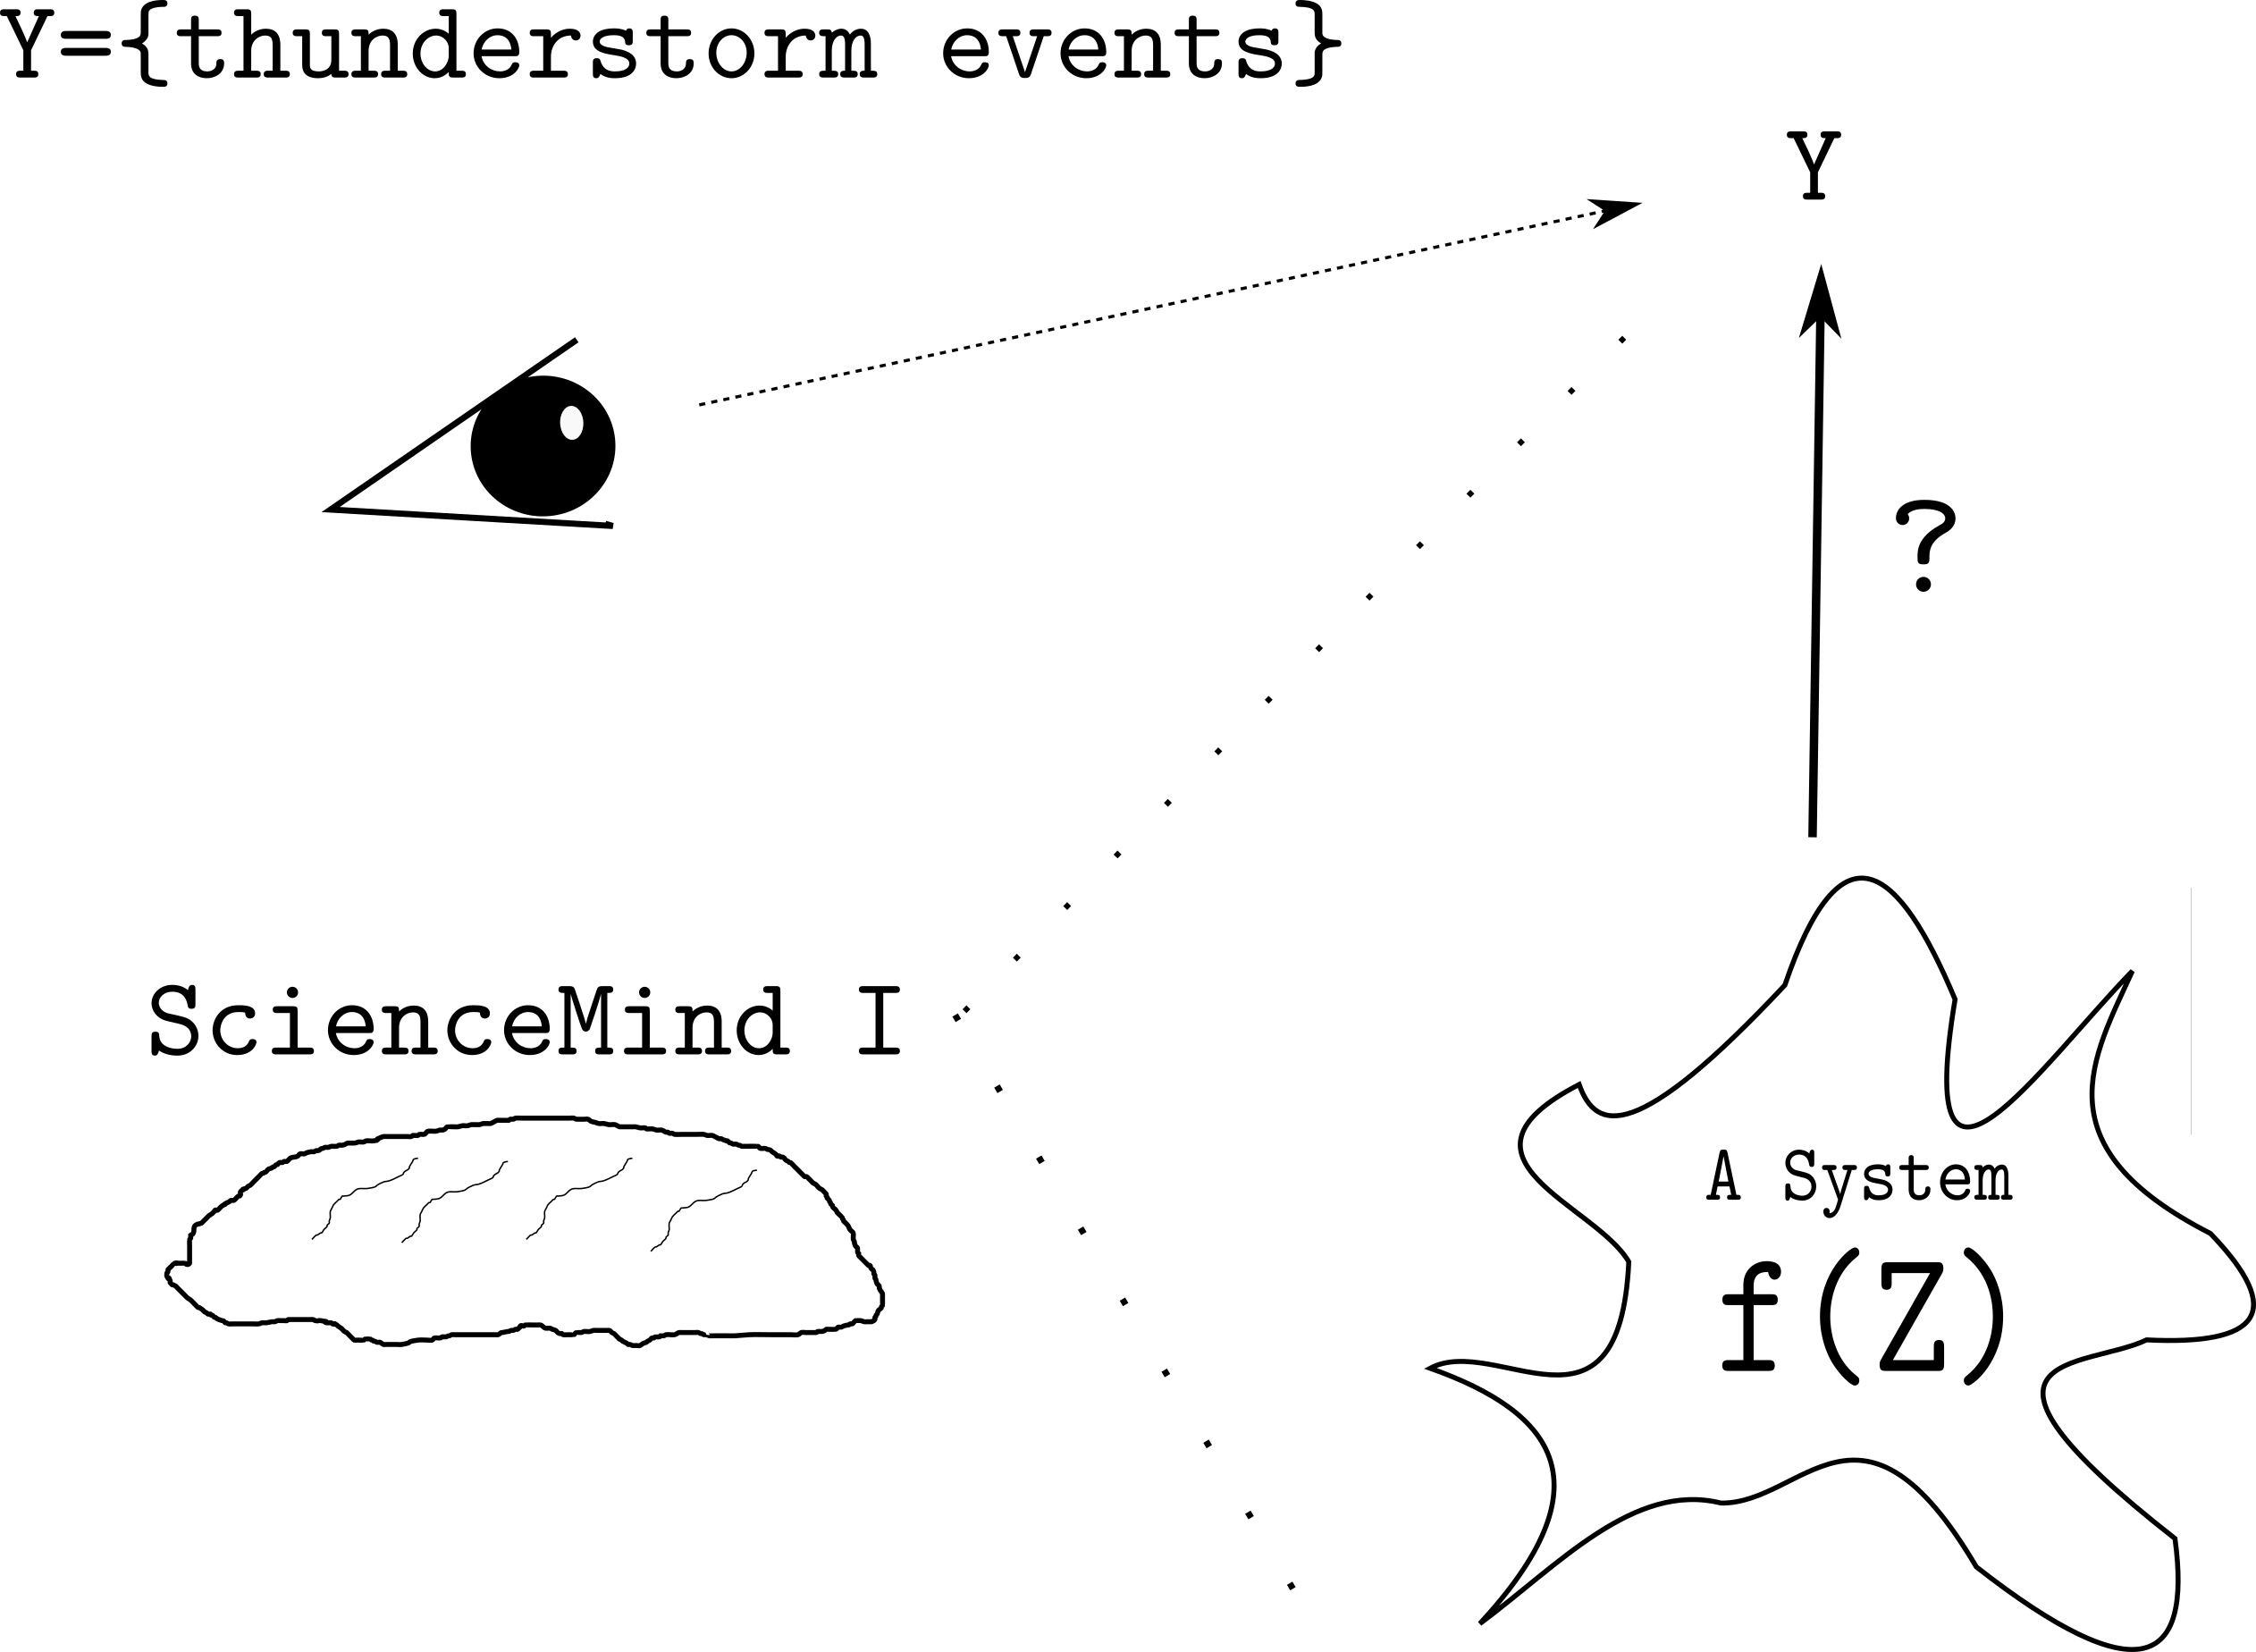
\includegraphics[scale=.75]{graphics/drawing1a}}; 
 \end{tikzpicture}

\end{frame}


%----------------------------------------------------------------
\begin{frame}

\begin{tikzpicture}[overlay]
  \node[anchor=south west] at (1.75,-5.25) {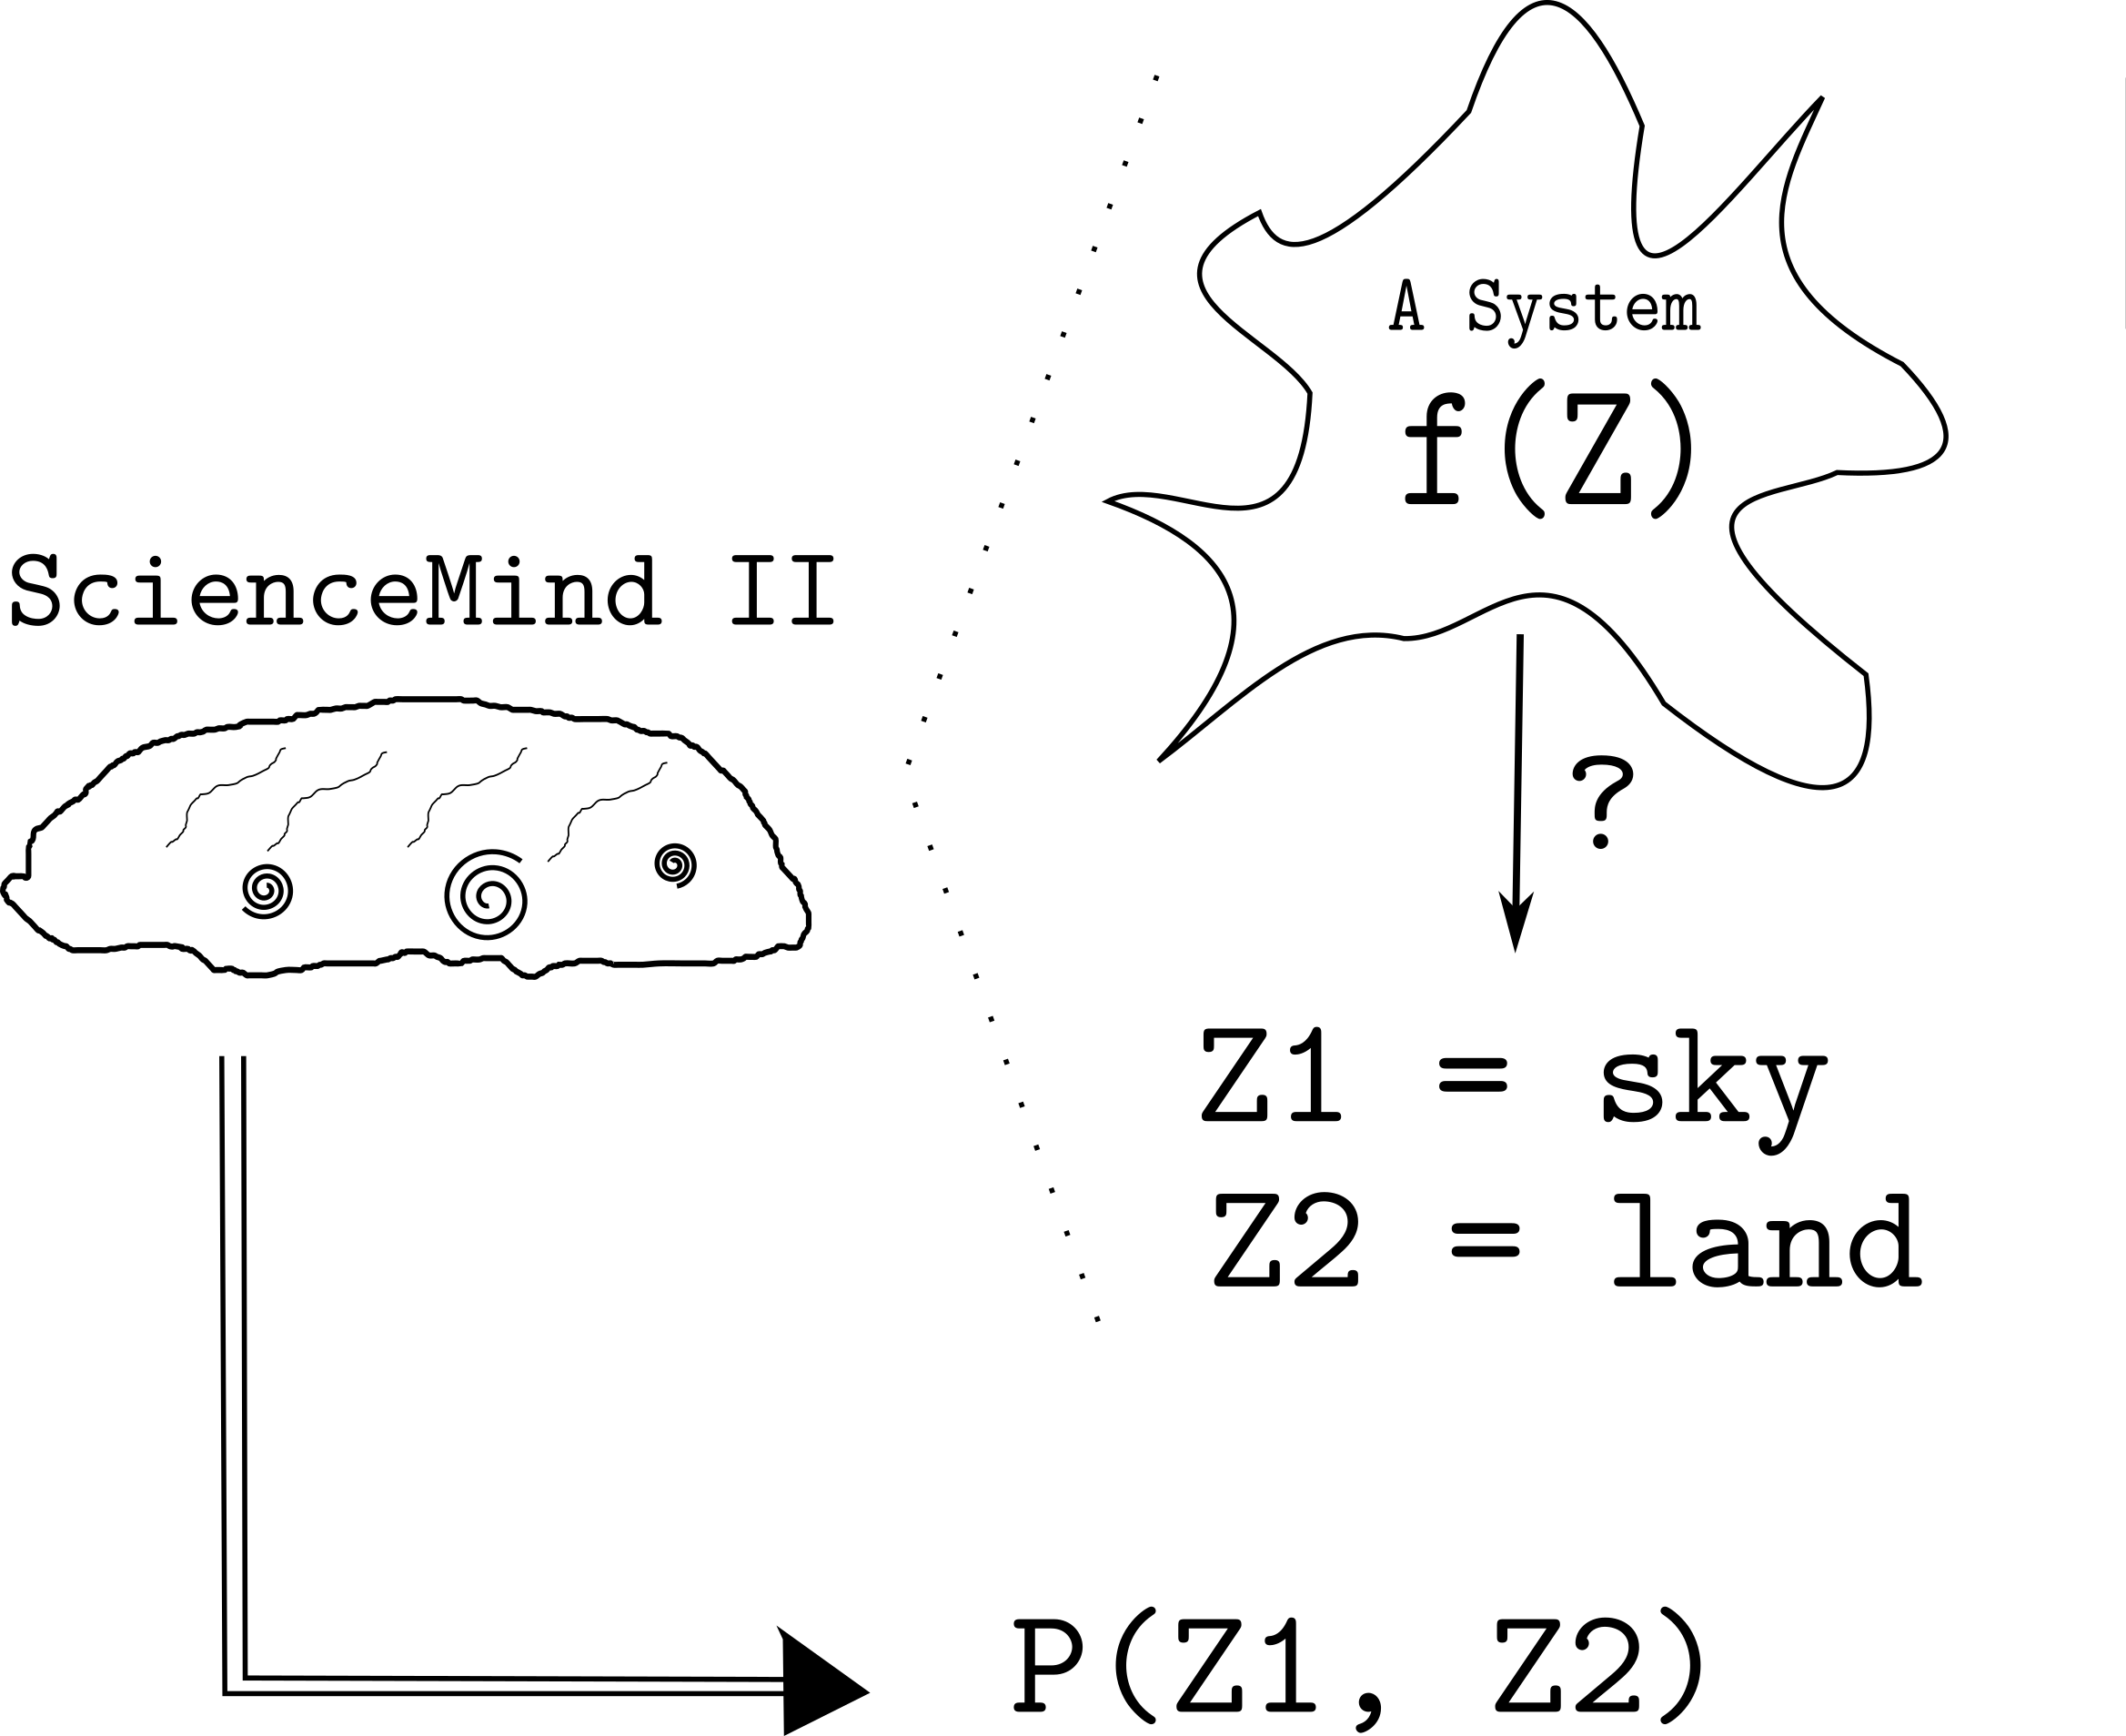
\includegraphics[scale=.70]{graphics/drawing1b}}; 
 \end{tikzpicture}

\end{frame}



%----------------------------------------------------------------
\begin{frame}

\begin{tikzpicture}[overlay]
  \node[anchor=south west] at (1.75,-5.25) {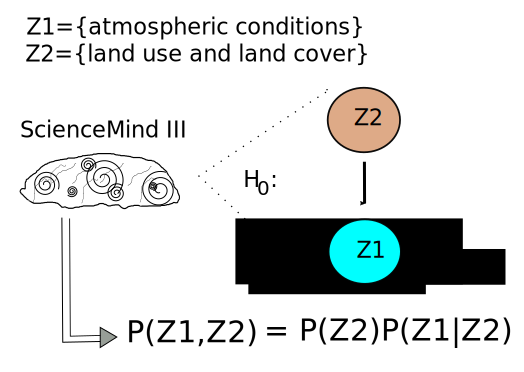
\includegraphics[scale=.70]{graphics/drawing1c}}; 
 \end{tikzpicture}

\end{frame}



%----------------------------------------------------------------
\begin{frame}

\begin{tikzpicture}[overlay]
  \node[anchor=south west] at (0.5,-1.0) {
\includegraphics[scale=.50]{graphics/Ashley1.jpeg}};
  \node[anchor=south west] at (0.5,-4.0) {
\includegraphics[scale=.50]{graphics/Stallins1.jpeg}};
 \end{tikzpicture}
 
 
 \begin{textblock}{1}(.5,.275)
  \small {... "substantive evidence of urban effects \\ 
  on thunderstorm frequency and severity" ...}
\end{textblock}

 \begin{textblock}{1}(.5,.55)
  \small {"Urban lightning research is still in the \\ 
  descriptive, pattern-identifying stage, \\
  with some inroads into mechanism."}
\end{textblock}

\end{frame}



%----------------------------------------------------------------
\begin{frame}

\begin{tikzpicture}[overlay]
  \node[anchor=south west] at (1.0,-5.5) {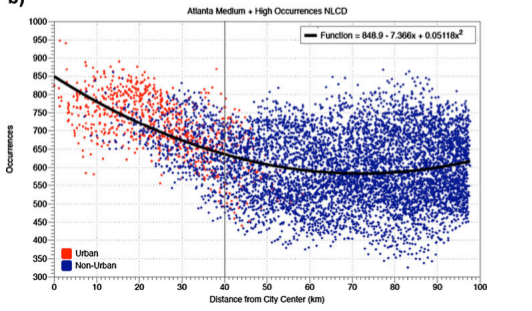
\includegraphics[scale=.75]{graphics/Ashley2.jpeg}}; 
 \end{tikzpicture}
 

\begin{textblock}{1}(.35,.125)
  \footnotesize {$P(Z1, Z2) \ = P(Z2)P(Z1|PZ2)$}
\end{textblock}

\begin{textblock}{1}(.15,.155)
  \footnotesize {$(dBZ = decibels \ radar \ reflectivity \Rightarrow  Z1; NLCD \ code \Rightarrow Z2)$}
\end{textblock}


\begin{textblock}{1}(.10,.20)
  \footnotesize{Occurrences $\geq 40$ dBZ for each 2-km grid cell vs. distance from city center}
\end{textblock}
 
 
\begin{textblock}{1}(.75,.72)
  \tiny {Ashley,Bentley,Stallins (2012)}
\end{textblock}

\end{frame}



%----------------------------------------------------------------
\begin{frame}

\begin{tikzpicture}[overlay]
  \node[anchor=south west] at (0,-2.0) {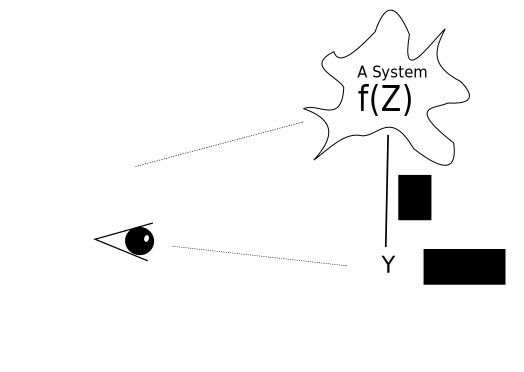
\includegraphics[scale=.35]{graphics/drawing2a}}; 
 \end{tikzpicture}
 
 
 \begin{textblock}{1}(0.40,.25)
  \scriptsize {
  \begin{itemize}
  	\item We observe an entity in Nature that we suspect \\
  	generates non-random patterns of information
  	\item Our states of knowledge about the causal relationships \\
  	and processes, $f(\cdot )$, that are operating as well as about \\
  	the inputs,	$Z$, are limited; often severely	
  	\item We assume that some observable outcome, $Y$, is \\
  	\underline{causally} related to the entity as $f(Z) \Longrightarrow \{Y\}$  	
  \end{itemize}
  }
 \end{textblock}

\end{frame}



%----------------------------------------------------------------
\begin{frame}

\begin{tikzpicture}[overlay]
  \node[anchor=south west] at (0,-2.0) {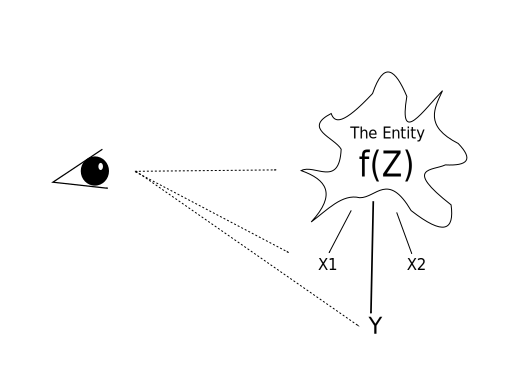
\includegraphics[scale=.35]{graphics/drawing3}}; 
 \end{tikzpicture}
 
 \begin{textblock}{1}(0.40,.25)
  \scriptsize {
  \begin{itemize}
  	\item We assume that some observable and measurable \\
  	attributes (data), $\{X1, X2\}$ are \underline{logically} related \\
  	 to the entity's internal processes as, $\{X1, X2\} | f(Z) $ 
  	\item Lacking full knowledge of the entity's processes, we use \\
  	a probability model and consider $X1, X2, Y$ as random \\
  	variables with a joint probability distribution function
  	\item Lacking complete datasets, we accept sampled datasets
  	\item We make inductive inferences from the sampled datasets \\
  	back to	$f(Z)$ by assuming sampling distributions, \\
  	evaluating our prior knowledge, and using the (weaker) \\
  	syllogisms of plausible reasoning coupled with probability \\
  	theory
  \end{itemize}
  }
 \end{textblock}

\end{frame}



%----------------------------------------------------------------
\begin{frame}



\end{frame}





%######################################
% END DOC
%######################################
\end{document}
